\chapter{Introduction}\label{chap:introduction}

\section{Motivation}
Instance detection is a critical task in computer vision, with applications ranging from autonomous driving to medical imaging. Despite significant advancements, unsupervised instance detection remains a challenging problem due to the lack of annotated data. This thesis aims to improve unsupervised instance detection by analyzing the problems with the current state-of-the-art unsupervised instance detection and segmentation methods.

In the field of Computer Vision, a significant shift has occurred from traditional Convolutional Neural Networks (CNNs) to the transformative capabilities of Transformers, as exemplified by the groundbreaking Vision Transformer (ViT) paper by Dosovitskiy et al. (2020)\cite{dosovitskiy2020image}. Subsequently, the concept of utilizing deep ViT features as dense visual descriptors was introduced by Amir et al. (2021)\cite{amir2021deep}, highlighting the strong semantic information these descriptors provide about instances within an image. Currently, the state-of-the-art method for unsupervised instance segmentation, CutLer, as proposed by Wang et al. (2023)\cite{wang2023cut}, employs DINO features\cite{caron2021emerging} as visual descriptors to effectively identify instances within images.

However, challenges such as the grouping of nearby instances, failure to identify complex background patterns, and the omission of small instances persist even in the current state-of-the-art methods. This thesis aims to investigate these failure cases, mainly based on the CutLer \cite{wang2023cut} baseline and propose methods to enhance the performance of unsupervised instance detection and segmentation tasks.

%\input{Images/main/mask_cut_cutler_comparison}
\begin{figure*}
	\centering
	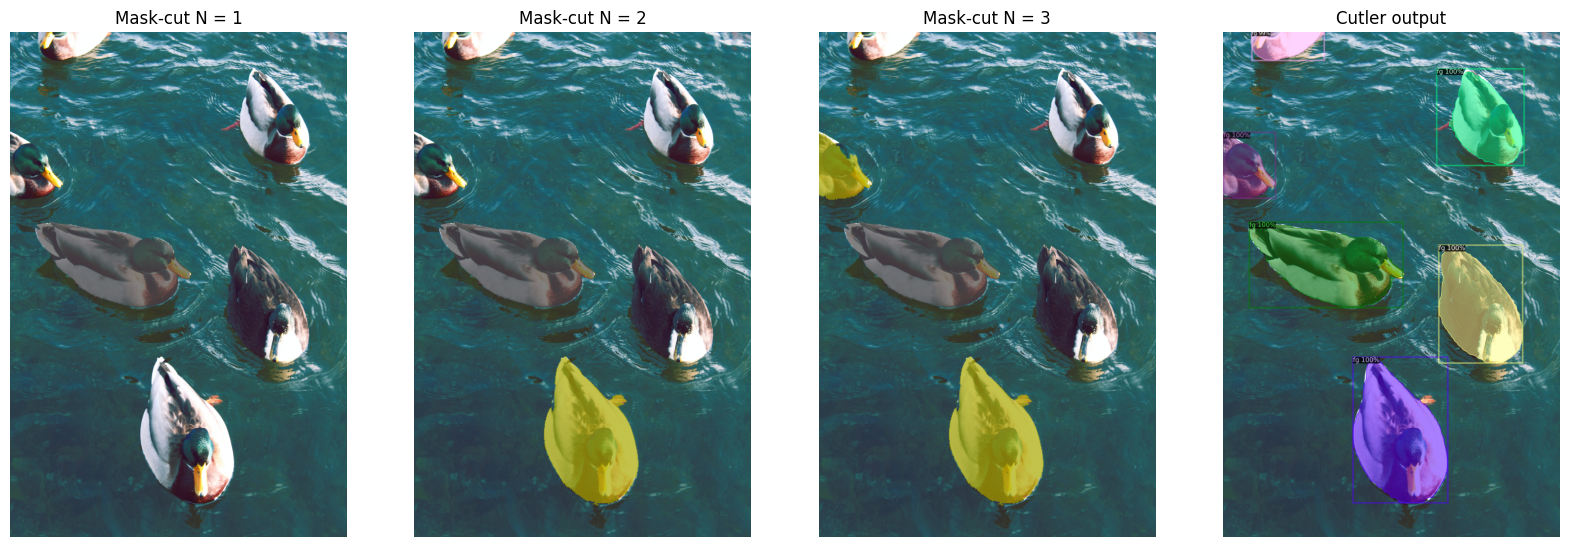
\includegraphics[width=1\textwidth]{Images/main/mask_cut_cutler_comparison.png}
	\caption[\textbf{Comparison of maskcut and CutLer outputs}]{\textbf{Comparison of maskcut and CutLer outputs}. Figure illustrates the outputs of CutLer and maskcut with different N(Number of mask generated) values.}
	\label{fig:mask_cut_cutler_comparison}
\end{figure*}

\section{Overview of CutLer}
In the field of unsupervised object detection and instance segmentation, the recent work by Xudong Wang et al. introduces Cut-and-LEaRn (CutLER)\cite{wang2023cut}, a novel approach that significantly advances the state-of-the-art. CutLER leverages the capabilities of self-supervised models to identify objects without human supervision, and it enhances this capability to train a high-performance localization model without any labeled data. The methodology begins with the MaskCut approach(inspired from \cite{wang2022tokencut}), which generates coarse masks for multiple objects within an image. Subsequently, a detector is trained on these masks using a robust loss function. Performance is further improved through a self-training process where the model is iteratively trained on its own predictions. This approach not only simplifies the training process but also proves to be compatible with various detection architectures and capable of detecting multiple objects simultaneously.

The effectiveness of CutLER is demonstrated through extensive evaluations across diverse image domains, including video frames, paintings, sketches, and complex scenes. Notably, CutLER, utilizing a ResNet50 backbone, achieves a substantial performance increase, more than doubling the detection accuracy on 10 out of 11 benchmarks compared to the previous state-of-the-art method, FreeSOLO, which uses a ResNet101 backbone. Specifically, CutLER improves the average precision (AP50) by over 2.7 times across these benchmarks. This demonstrates CutLER's potential not only as a zero-shot unsupervised detector but also as an efficient low-shot detector, marking a significant step forward in unsupervised object detection and instance segmentation.

\section{Contribution and Key Insights}

This study focuses on the shortcomings of CutLer and the methods to minimize them. Our main contributions are:

\begin{enumerate}
    \item \textbf{Analysis on the performance of different metrics for discriminating instances}: We compare the effectiveness of distance and similarity measures on discriminating instances of same and different classes.
    +
    \item \textbf{Analysis on the influence of overlapping instances}: We compare the performance of the model when trained with and without overlapping instances and conclude that training without overlapping instances results in better instance discrimination.

    \item \textbf{Refining maskcut masks}: On top of self training, ee refine mask-cut masks using CutLer output to remove noisy masks and retraining to yield better performance.
\end{enumerate}

% Wite about the improvement
%These contributions collectively elevate the understanding and practical implementation of GroupViT, opening doors to broader applications. Notably, the research achieves 18\% improvement on the training dataset, maintaining strong results on downstream datasets like PASCAL VOC and PASCAL Context.

\section{Outline}
\begin{itemize}
    \item \textbf{Chapter \ref{chap:relatedwork}:} %Explores semantic segmentation in the context of deep learning, with a focus on addressing challenges through weak supervision. Introduces the concept of open vocabulary segmentation and provides an overview of Unsupervised Segmentation.
    
    \item \textbf{Chapter \ref{chap:background}:} %Delves into the foundational aspects of Transformers, with a special emphasis on the attention mechanism crucial for understanding GroupViT. Also introduces key components of DINO.
    
    \item \textbf{Chapter \ref{chap:approach}:} %Provides an in-depth discussion of GroupViT, including a detailed explanation of entropy regularization techniques.
    
    \item \textbf{Chapter \ref{chap:experiments}:} %Details various experiments, starting with the fine-tuning process and progressing to explore entropy regularization and noise-free contrastive loss. The chapter concludes by discussing attempts to integrate DINO features into GroupViT. These experiments reveal an effective method for fine-tuning GroupViT on smaller, cleaner datasets while maintaining strong downstream performance.
\end{itemize}